Nesse capítulo fazemos uma revisão bibliográfica da área de Dinâmicas de
Opinião\footnote{Doravante OD (\textit{Opinion Dynamics}).} Definimos a área, o
que são modelos baseados em agente e quais os constituintes típicos de um modelo
de OD. Depois apresentamos modelos que podem ser considerados canônicos, em sua
versão mais simples, pelo fato de inspirarem uma gama de modificações e
extensões. Na seção seguinte discutimos algumas questões teóricas referentes à
atualização da opinião dos agentes e concluímos o capítulo com uma discussão de
nossa abordagem.


\section{Definição da Área}

OD é uma área que pode ser definida a partir de 3 elementos. Primeiramente,
sistemas alvo em comum, delimitados pela pergunta central: quais elementos
determinam se um grupo de agentes chega ao consenso sobre algo, ou ao invés
disso persistem em discórdia? \cite{castellano2012social}\footnote{Essa pode ser
  pensada como a pergunta \textit{fundacional} da área \cite{flache2017}.}.
Segundo, um conjunto de modelos que partilham elementos constitutivos,
particularmente fazendo uso da técnica da Modelagem Baseada em
Agentes\footnote{De agora em diante vamos usar a abreviação ABM para modelagem
  (ou modelo(s)) baseada(os) em agentes.}, e em, alguma medida, de
\textit{insights} e técnicas da Física Estatística \cite{galam1990social}.
Terceiro, uma comunidade de pesquisadores que partilham do interesse no objeto,
fazem uso de referenciais e técnicas compartilhadas e se reconhecem como membros
dessa comunidade.

Na área há a aceitação de um significado amplo e abstrato de opinião como uma
característica de um agente que pode ser mudada com pouco custo
\cite[p.312]{castellano2012social}. Isso permite com que ela vise sistemas alvos
tais como voto, ciência, cultura, difusão de tarifas, dentre outros
\cite{kowalska2013going,martins2015thou,axelrod1997dissemination,galam1990social}.
Essa gama de aplicações está relacionada com a base disciplinar dos pesquisadores,
envolvendo pessoas de áreas como Física, Sociologia, Ciência Política, Economia,
Psicologia Social, dentre outras, o que nos permite considerar a área como um
subgrupo da Sociofísica \cite{galam1982sociophysics,galam2012sociophysics}.


\section{Modelagem Baseada em Agentes e Dinâmicas de Opinião}

Modelos Baseados em Agentes podem ser definidos como modelos que envolvem
agentes discretos, onde agentes, seus atributos, e possivelmente um ambiente são
definidos algoritmicamente \cite{sayama2015introduction} \footnote{ ABMs
  costumam ser implementados como simulações num computador, embora existam
  modelos baseados em agentes que historicamente não tenham sido diretamente em
  computadores, como os modelos de Schelling e de Sakoda
  \cite{hegselmann2017thomas}.}. Num ABM existem três noções primitivas: os
\textit{atributos}, os \textit{estados} e as \textit{configurações}
\cite{de2014agent}. Os atributos dos agentes são o conjunto de propriedades
que cada cada agente \(i\) tem. Os estados dos agentes são os valores de seus
atributos num determinado tempo \(t\). Já as configurações são as coleções de
todos os estados dos agentes num modelo.

ABM é uma técnica flexível: podemos construir modelos ``metafóricos'' com
objetivo de auxiliar o desenvolvimento de intuição segundo a elucidação de
princípios; ou de alta-fidelidade, com dezenas de atributos e um
ambiente incluindo casas, escolas, sistemas de transporte, dentre outros, com o
objetivo avaliar contrafactuais próximos a determinados casos concretos
\cite{de2014agent, epstein2006generative}.


Segundo \citeonline[p.430-1]{sayama2015introduction}, ABMs têm as seguintes
propriedades típicas:
\begin{itemize}
\item agentes podem ter estados internos;
\item agentes podem ser espacialmente localizados;
\item agentes podem perceber e interagir com o ambiente;
\item agentes podem interagir segundo regras pré-definidas;
\item agentes podem ser capazes de aprender e adaptar-se;
\item agentes podem interagir com outros agentes;
\item AMBs muitas vezes não tem supervisores/controladores centrais;
  \item ABMs podem produzir comportamentos coletivos não triviais.
  \end{itemize}

  Tendo em vista essas propriedades, ABMs são particularmente úteis para o
  estudo de sistemas complexos \cite{wilensky2015introduction}, dada: sua
  capacidade de incluir redes e espaço; seu potencial de ligar múltiplos
  domínios e de incluir uma maior heterogeneidade de agentes; além de seu foco
  na robustez de resultados \cite{de2014agent,wilensky2015introduction}. Não por
  acaso, ABMs são amplamente usados em OD  \cite{castellano2012social,flache2017}.

  Que elementos constituem os modelos de OD ? Podemos delimitar um modelo de
  dinâmicas de opinião da seguinte forma: agentes,conectados, possuem opiniões
  como variáveis e interagem segundo regras que explicam a mudança ou manutenção
  das opiniões individuais sob efeito da interação com outros agentes ou outras
  fontes (como a mídia) \cite{sirbu2017opinion}. Os agentes num modelo em OD têm
  então : uma \textit{opinião}; uma \textit{estrutura de interação}; e uma
  \textit{regra de atualização} de sua opinião.


  A opinião dos agentes pode ser representada como uma variável ou conjunto de
  variáveis, que por sua vez podem ser discretas ou contínuas. Já a estrutura de
  interação consiste no conjunto de agentes cujas ações e propriedades podem
  afetar a opinião de um agente \(i\) \cite{page2008uncertainty}.

  Podemos dividir a estrutura de interação numa \textit{topologia} de interação e
  numa \textit{regra de interação}. A topologia de interação define quais
  agentes estão conectados com \(i\), e podem, potencialmente, afetá-lo. A regra
  de interação define como \(i\) interage com os agentes desse conjunto(seus
  ``vizinhos''). Em OD as regras de interação definem qual a
  relação que o agente \(i\) tem com seus vizinhos: se interage com um vizinho
  por vez, uma interação em díade, ou com algum subconjunto de seus vizinhos,
  uma interação em grupo. Por fim, a regra de atualização define sob qual regra
  a opinião do agente \(i\) muda do tempo \(t\) para o tempo \(t+1\). 

  

  \section{Modelos Canônicos}

  Adaptações do Modelo de Ising são os modelos mais fundamentais na área. O
  modelo de Ising é um modelo paradigmático da Mecânica Estatística, usado para
  representar o processo de magnetização de materiais\footnote{O modelo de Ising
    é um modelo paradigmático de sistemas com muitas partes interagindo levando
    à uma transição de fase, a uma mudança de comportamento qualitativo do
    sistema. Sendo assim, é aplicado em vários contextos além da sua concepção
    original, como mercados financeiros, sistemas ecológicos, e dinâmicas de
    opinião \cite{sole2011phase}}. Neles, variáveis discretas, \textit{spins},
  com valores $s = \pm 1$, estão localizadas num grafo, e têm uma tendência a
  alinhar-se com seus vizinhos: se a maioria tem \(s = + 1 \) o spin muda seu
  valor para \(+1\); se a maioria tem \(s = -1 \) o spin muda seu valor para
  \(-1\); se houver empate o spin muda seu valor com probabilidade
  \(\frac{1}{2}\) \cite{castellano2012social,sole2011phase}. A reinterpretação
  para o contexto de OD é o seguinte: o spin é um agente; sua opinião pode ter
  os valores \(+1\) ou \(-1\); um agente interage com todos seus vizinhos por
  passo de tempo; ele assume a opinião da maioria deles.

  Um modelo parecido com o anterior é o ``Voter'' \cite{holley1975ergodic}. Nele
  cada agente tem uma opinião binária \(\pm\) 1 ; e a cada passo um agente é
  selecionado aleatoriamente e assume a opinião de algum de seus vizinhos.
  Difere do modelo anterior, portanto, na regra de interação, díade ao invés do
  grupo inteiro, e de atualização, assume o valor do vizinho ao invés da maioria
  deles.


  Já no modelo da Regra de Maioria  a interação é : a cada
  ``tick'' um grupo de tamanho \textit{r} é selecionado aleatoriamente e todos
  os agentes mudam sua opinião para a opinião da maioria do grupo
  \cite{galam1990social,galam2012sociophysics}. O tamanho \textit{r} pode ser
  fixo ou ser tirado de alguma distribuição a cada passo. Se \textit{r} for par
  podem ocorrer empates nos grupos, de forma que ou o grupo escolhe uma das
  opiniões com probabilidade \(\frac{1}{2}\), ou introduz-se um viés, e toda vez
  que houver empate o grupo muda para uma das opiniões
  \cite{galam2012sociophysics, galam1986majority}.

  O Modelo Sznajd também é bastante discutido na literatura
  \cite{sznajd2000opinion, sirbu2017opinion,castellano2012social}. Nele cada
  agente têm exatamente dois vizinhos, em uma grade unidimensional. A cada passo
  um par $ij$ de vizinhos é selecionado e se sua opinião for igual os outros
  vizinhos de \(i\) e \(j\) mudam a opinião para a opinião de convergência. Se
  eles discordarem, \(i\) adota a opinião do outro vizinho, e \(j\) faz o mesmo.

  Todos os modelos até agora representaram opiniões como uma variável que pode
  tomar valores binários. Além disso a regra de atualização dos modelos
  pressupõe uma interação assimilativa: indivíduos conectados por meio de uma
  relação estrutural influenciam uns aos outros em direção à diminuição da
  diferença de suas opiniões \cite{flache2017}. O modelo de
  \citeonline{axelrod1997dissemination} difere em ambos os aspectos. Cada agente
  tem por opinião um vetor $F$ de componentes $(\sigma_1 , \ldots, \sigma_f)$
  \cite{klemm2003role}. Esses $\sigma_i$ podem tomar valores inteiros de 0 a 9. Os
  componentes são as características culturais dos agentes e seus possíveis
  valores são seus traços culturais \cite{gomes2014}. O modelo considera
  interação entre pares de vizinhos, os quais interagem com uma probabilidade
  proporcional ao número de traços que têm igual. Isso significa que se \(i\)
  tem uma opinião igual a 82330 e seu vizinho \(j\) tem uma opinião 67730 eles
  têm \(40 \%\) de interagirem. Se eles interagirem, \(i\) troca um dos traços
  em que difere \(por\) j um dos traços de
  \(j\)\cite{axelrod1997dissemination}. Nesse modelo pessoas similares
  têm uma probabilidade maior de se interagirem do que pessoas distintas, mas
  uma vez que a interação ocorre elas ficam mais parecidas. Sendo assim, o
  modelo de Axelrod pode ser considerado um modelo de assimilação enviesada: só
  indivíduos suficientemente similares podem influenciar uns aos outros na
  redução de suas diferenças \cite{flache2017}.


Um outro modelo canônico de assimilação enviesada é o Modelo de
Deffuant-Weisbuch \cite{deffuant2000mixing}. Nele cada agente \(i\) tem opinião
inicial \( o_i \in [0,1]\). Dois agentes são escolhidos aleatoriamente, e \(i\) é
influenciado por \(j\) se \(| o_i - o_j| < \epsilon\). Se isso ocorrer suas opiniões se
aproximam de acordo com um parâmetro $0 < \mu< \leq 0.5$, de forma que: $o_{i,t+1} =
o_{it} + \mu(o_{jt} - o_{it})$. Esse modelo é particularmente relevante para o
presente trabalho, por duas razões: a opinião é contínua, assim como a
representação das ``utilidades'' dos agentes em Teoria Política Espacial
\footnote{Na verdade, ligar a literatura de OD com funções de utilidade em
  economia e com a noção geométrica de política é a justificativa dada por
  \citeonline{deffuant2000mixing} para considerar opiniões como contínuas.}; e
\(\epsilon\) pode ser interpretado como parte da regra de atualização, o que faz modelo
os agentes tenham viés de confirmação.

Quando \(\epsilon\) é interpretado como parte da regra de interação temos o princípio
da homofilia: padrões estruturais de interação social levam pessoas a ter maior
probabilidade de interagirem com pessoas similares a elas
\cite{mcpherson2001birds}. Quando \(\epsilon\) é interpretado como parte da regra de
atualização temos o fenômeno do \textit{viés de confirmação}: a tendência das
pessoas de dar maior peso a informações que confirmem suas crenças anteriores
\cite{nickerson1998confirmation}.

\citeonline{huckfeldt2005patterns} argumenta que indivíduos escolhem redes de
discussão com razões distintas às políticas (como interesses profissionais e
hobbies) e acabam interagindo com indivíduos cujas filiações partidárias
distintas. Desta forma, o papel da homofilia em política é atenuado. Já o
\textit{vies partidário} dos cidadãos, o viés de confirmação no tocante a
questões políticas , é um resultado estabelecido na literatura em opinião
pública e psicologia política, e imprescindível para a modelagem generativa de
opinião pública \cite{bartels2002beyond, flynn2017nature,
  lodge2013rationalizing}.


\section{Regra de Atualização e Processamento de Informação}


Como lembra Dirk Helbing, não existe uma única forma de modelar agentes
interagindo em sistemas sociais complexos \cite{helbing2010pluralistic}. Os
modelos canônicos em OD têm uma abordagem que Helbing chama de
\textit{fisicalista}: abstraem as interações sociais ao ponto delas poderem ser
estudadas como um modelo de ``partículas''. Em OD essa abordagem é refletida na
forma como se modela a regra de atualização: abstrai-se o processamento de
informação, a cognição dos agentes. Isso, como frisa Helbing, não é uma falha
dos modelos. Paul Ormerod defende que o \textit{null model} em sistemas sociais
complexos deveria ser o de um \textit{zero intelligence actor}, pois a
complexidade dos sistemas nos permitiria modelar os agentes ``como se fossem''
átomos \cite{ormerod2008can, bentley2012agents}.

Não obstante, um conjunto de trabalhos em OD tem buscado abrir a ``caixa-preta''
da cognição dos agentes e tratam a atualização de opinião como resultado de um
processamento de informação explicitamente modelado \cite{flache2017,
  jager2017}. O modelo Polias de \citeonline{brousmiche2016beliefs}, o modelo
Innomind de \citeonline{schroder2017modeling} e o modelo Lodge-Taber
\cite{kim2010computational,kim2011model} de processamento dual e raciocínio
motivado são exemplos dessa tendência.

Se pensarmos num espectro possível de abordagens para a cognição dos agentes,
ilustrado na Figura 5, esses modelos estão posicionados no extremo oposto aos
modelos fisicalistas. Enquanto os modelos fisicalistas abstraem totalmente o que
se passa na cabeça dos agentes os modelos (neuro)cognitivos buscam representar a
arquitetura cognitiva que alicerça as atitudes e crenças
deles\cite{kim2010computational}.

\todo[inline,color = yellow]{Discutir melhor o que é uma
  arquitetura cognitiva?}

\begin{figure}[H]
  \centering
  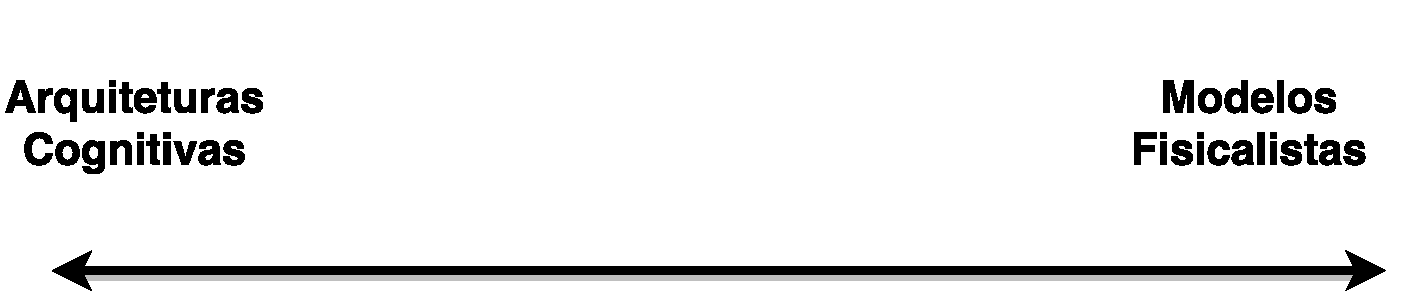
\includegraphics[width = \textwidth, height = 3cm]{ims/line.pdf}
  \caption{Espectro de abordagens no tocante à cognição dos agentes}
  \label{fig5}
\end{figure}

Modelos cognitivamente ``densos'' permitem que analisemos como processos de
influência social estão micro-fundamentados em processos mentais subjacentes, e
é um fronte dentre os trabalhos que buscam aumentar o realismo das simulações
sociais \cite{jager2017,epstein2014agent_zero, conte2013minding}. Contudo, como
argumenta Jonathan Bendor, na medida em que a Ciência Política busca modelar
macrofenômenos ela ``deve ser mais implacável em relação à micropressupostos do
que microcampos relacionados (como ciência cognitiva)''
\cite[p.45]{bendor2010bounded}. Quanto mais complicados nossos modelos menor
controle temos sobre qual o elemento responsável pelo seus resultados, e mais
dados precisamos para a sua calibração e validação \cite{de2005computational}.
Como canonicamente argumentado por \citeonline{zaller1992nature}, a estratégia
metodológica para modelar a opinião pública, um fenômeno social de larga escala,
envolve incorporar no modelo somente os aspectos do processamento de informação
que têm relevância para a compreensão das dinâmicas do fenômeno, ao invés de
buscar desenvolver modelos que aproximam o mais próximo o possível os detalhes
da mente humana\footnote{No contexto da análise institucional um argumento
  equivalente é feito por \citeonline{ostrom1990governing}.}.


\citeonline{martins2012bayesian} apresenta um \textit{framework} para modelar
Dinâmicas de Opinião que é cognitivamente mais
``denso''\footnote{\textcolor{red}{Eu não sei qual o termo usar aqui, agradeço
    sugestões}. } que os modelos fisicalistas, mas sem buscar modelar as bases
neurocognitivas de processamento de informação. O \textit{framework} está
fundamentado no uso da inferência bayesiana como base da regra de atualização
dos agentes. Embora seja bem documentado que as pessoas não seguem fielmente o
princípio da racionalidade bayesiana, apresentado no primeiro capítulo, um
conjunto de trabalhos em psicologia e ciência cognitiva vêm, nos últimos anos,
defendendo a possibilidade de que sejamos ``bayesianos
imperfeitos''\cite{griffiths2006optimal,fujikawa2007perfect,baker2017rational,
  gintis2016individuality}. Usar um framework bayesiano é, desta forma, uma
aproximação e permite a construção de modelos de dinâmicas de opinião de uma
forma fundamentada num princípio comum, algo particularmente relevante numa área
em que há a proliferação de modelos ad-hoc \cite{flache2017,jager2017}.

 \citeonline[p.214]{martins2012bayesian} oferece o seguinte passo a passo
para a construção de um modelo de dinâmicas de opinião com base num
\textit{framework} bayesiano:

\begin{enumerate}
\item Identificar uma questão sob debate e chamá-la de $x$. \(x\) pode ser
  discreto ou contínuo.
\item cada agente \(i\) tem uma opinião subjetiva sobre $x$ e essa opinião é
  representada pela distribuição de probabilidade $f_i(x)$ .
\item Ocorre comunicação : a comunicação é a declaração de um valor
  $ A_j$ pelo agente $j$ de tal forma que $A_j[f]$ é um funcional de
  $f_j(x)$.
\item Os agentes tem que ter em sua mente  uma relação entre o
  verdadeiro valor entre $x$ e o valor declarado $A_j$. Isso é dado
  pela distribuição de probabilidade $P(A_j|x)$.
\item Dado o prior $f_i(x)$ a opinião posterior $f_i(x|A_j)$ é dada
  por $A_i[f_i(x|A_j)]$ que é a nova opinião de $i$ .
\end{enumerate}


\todo[inline,color = yellow]{Discutir o CODA aqui??}


A aplicação desse \textit{framework} no caso de opiniões contínuas incorpora o
mecanismo de viés de confirmação presente no modelo  Deffuant-Weisbuch,
recupera seus resultados qualitativos, e ainda tem resultados adicionais
\cite{martins2009bayesian}. Dado que o modelo representa a atualização de uma
variável contínua, incorpora viés de confirmação e fundamenta a regra de
atualização num framework bayesiano de processamento de informação será a base
do nosso trabalho e será discutido no Capítulo 3.


